\section{Epidemien - Logistisches Modell}
\label{sec:epidemiology-logisitc-model}

\begin{code}
	\caption{Skript für die Simulation mit einem logistischen Modell}
	\mSourceFile{\srcDir/epidemiologyLogisitcProg.m}
	\label{source:epidemiology-logistic-program}
\end{code}

\begin{code}
	\caption{Funktion zur Berechnung des logistischen Modell}
	\mSourceFile{\srcDir/epidemiologyLogisitc.m}
	\label{source:epidemiology-logistic}
\end{code}

\begin{figure}[h]
	\centering
	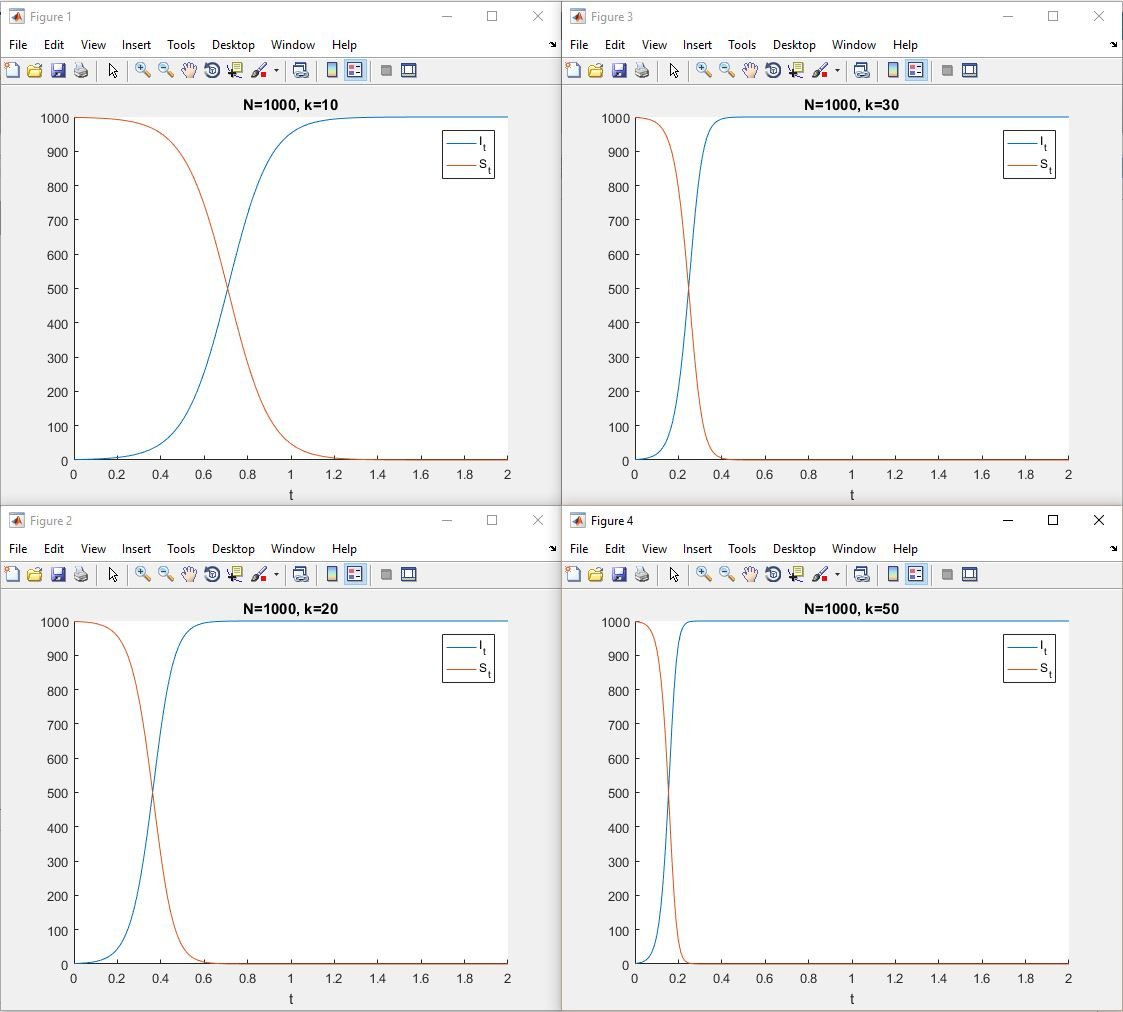
\includegraphics[scale=0.55]{\imageDir/epiomology-logistic.JPG}
	\caption{Verlauf der Epidemie mit einem logistischen Modell}
	\label{test:epidemiology-logistic}
\end{figure}
\ \newline
Je kleiner $k$ ist, desto länger braucht die Epidemie zum Ausbrechen und desto länger dauert die Epidemie an, wobei der Verlauf der Epidemie gegenüber einem größeren $k$ flacher ist. Bei einem größeren $k$ bricht die Epidemie schneller aus und hat einen steileren Verlauf.
